\documentclass[margin=10pt]{standalone}

\usepackage{tikz}

\usetikzlibrary{decorations.pathreplacing,arrows,shapes,positioning,shadows,calc}

\begin{document}

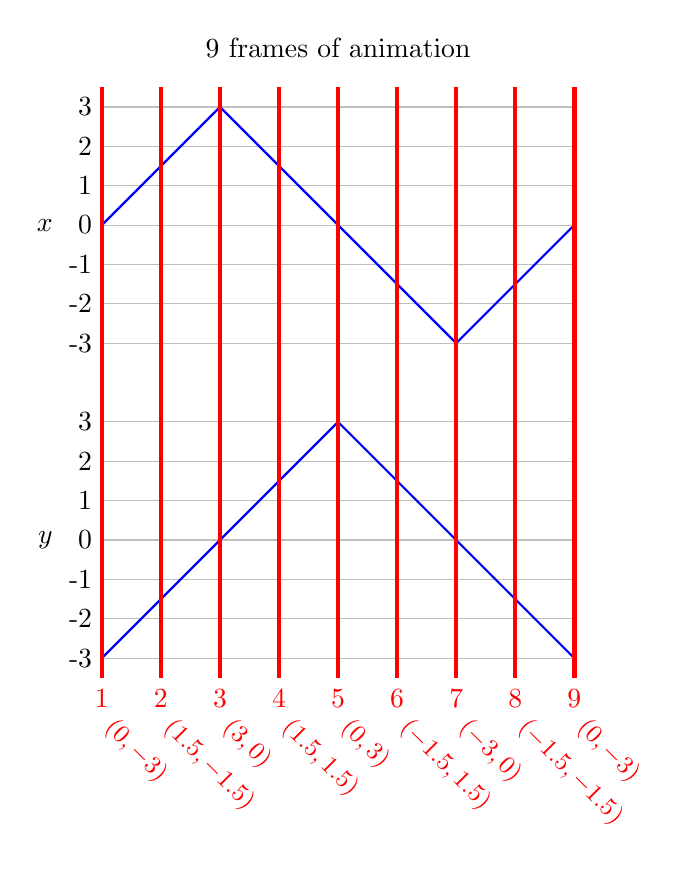
\begin{tikzpicture}[scale=0.5]
%	\draw (0,0) rectangle (10,7);
	\draw (0,0) node[anchor=north] {9 frames of animation};
	
	\begin{scope}[shift={(-6,-5)}]
		\draw (0,-3) -- (0,3);
		
		\draw (-1,0) node[anchor=east] {$x$};

		\draw (0,-3) node[anchor=east] {-3};
		\draw (0,-2) node[anchor=east] {-2};
		\draw (0,-1) node[anchor=east] {-1};
		\draw (0,0) node[anchor=east] {0};
		\draw (0,1) node[anchor=east] {1};
		\draw (0,2) node[anchor=east] {2};
		\draw (0,3) node[anchor=east] {3};
		
		\draw[lightgray] (0,-3) -- ++ (12,0);
		\draw[lightgray] (0,-2) -- ++ (12,0);
		\draw[lightgray] (0,-1) -- ++ (12,0);
		\draw[lightgray] (0,0) -- ++ (12,0);
		\draw[lightgray] (0,1) -- ++ (12,0);
		\draw[lightgray] (0,2) -- ++ (12,0);
		\draw[lightgray] (0,3) -- ++ (12,0);
		
		\draw[thick,blue] (0,0) -- (3,3) -- (9,-3) -- (12,0);
	\end{scope}
	
	\begin{scope}[shift={(-6,-13)}]
		\draw (0,-3) -- (0,3);
		
		\draw (-1,0) node[anchor=east] {$y$};

		\draw (0,-3) node[anchor=east] {-3};
		\draw (0,-2) node[anchor=east] {-2};
		\draw (0,-1) node[anchor=east] {-1};
		\draw (0,0) node[anchor=east] {0};
		\draw (0,1) node[anchor=east] {1};
		\draw (0,2) node[anchor=east] {2};
		\draw (0,3) node[anchor=east] {3};
		
		\draw[lightgray] (0,-3) -- ++ (12,0);
		\draw[lightgray] (0,-2) -- ++ (12,0);
		\draw[lightgray] (0,-1) -- ++ (12,0);
		\draw[lightgray] (0,0) -- ++ (12,0);
		\draw[lightgray] (0,1) -- ++ (12,0);
		\draw[lightgray] (0,2) -- ++ (12,0);
		\draw[lightgray] (0,3) -- ++ (12,0);
		
		\draw[thick,blue] (0,-3) -- (6,3) -- (12,-3);
	\end{scope}
	
	\begin{scope}[shift={(-6,-1.5)}]
		\draw[ultra thick,red] (0,0) -- ++ (0,-15) node[anchor=north] {1};
		\draw[ultra thick,red] (1.5,0) -- ++ (0,-15) node[anchor=north] {2};
		\draw[ultra thick,red] (3,0) -- ++ (0,-15) node[anchor=north] {3};
		\draw[ultra thick,red] (4.5,0) -- ++ (0,-15) node[anchor=north] {4};
		\draw[ultra thick,red] (6,0) -- ++ (0,-15) node[anchor=north] {5};
		\draw[ultra thick,red] (7.5,0) -- ++ (0,-15) node[anchor=north] {6};
		\draw[ultra thick,red] (9,0) -- ++ (0,-15) node[anchor=north] {7};
		\draw[ultra thick,red] (10.5,0) -- ++ (0,-15) node[anchor=north] {8};
		\draw[ultra thick,red] (12,0) -- ++ (0,-15) node[anchor=north] {9};
		
		\draw[red] (0,-16) node[anchor=west, rotate=-45] {\small $(0,-3)$};
		\draw[red] (1.5,-16) node[anchor=west, rotate=-45] {\small $(1.5,-1.5)$};
		\draw[red] (3,-16) node[anchor=west, rotate=-45] {\small $(3,0)$};
		\draw[red] (4.5,-16) node[anchor=west, rotate=-45] {\small $(1.5,1.5)$};
		\draw[red] (6,-16) node[anchor=west, rotate=-45] {\small $(0,3)$};
		\draw[red] (7.5,-16) node[anchor=west, rotate=-45] {\small $(-1.5,1.5)$};
		\draw[red] (9,-16) node[anchor=west, rotate=-45] {\small $(-3,0)$};
		\draw[red] (10.5,-16) node[anchor=west, rotate=-45] {\small $(-1.5,-1.5)$};
		\draw[red] (12,-16) node[anchor=west, rotate=-45] {\small $(0,-3)$};
	\end{scope}
\end{tikzpicture}

\end{document}